\section{Kinematics}

\begin{figure}[h]
    \begin{minipage}{0.49\textwidth}
        \begin{figure}[H]
            \centering
            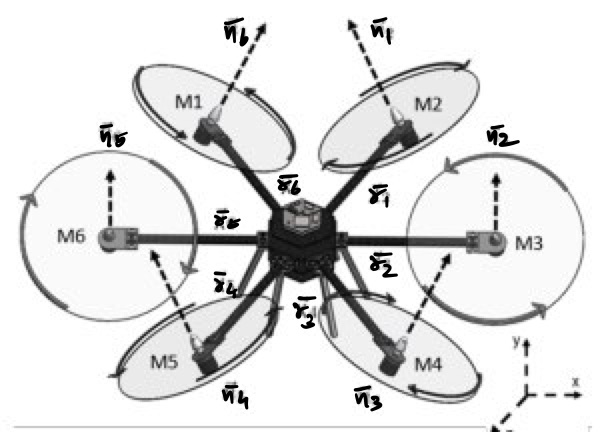
\includegraphics[width = 0.9\textwidth]{./figs/hex_copt-1.jpg}
        \end{figure}
    \end{minipage}
        \begin{minipage}{0.49\textwidth}
        \begin{figure}[H]
            \centering
            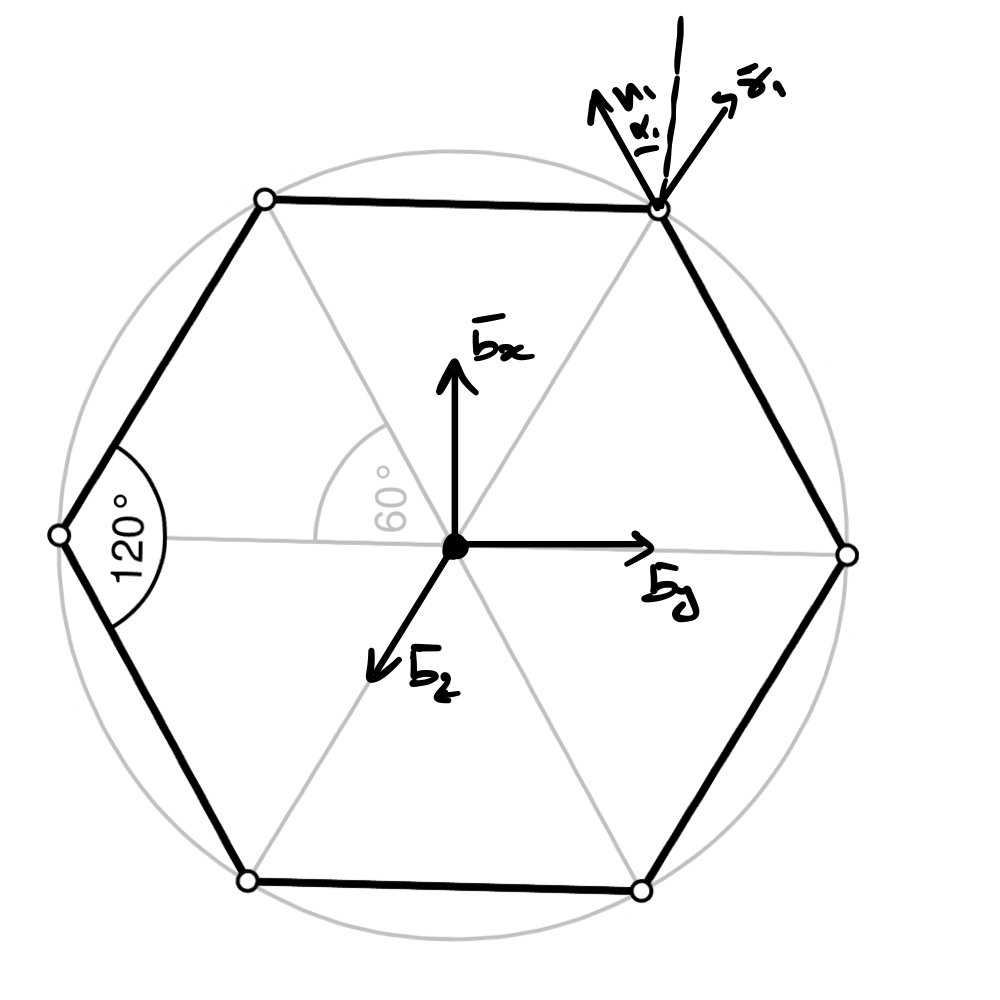
\includegraphics[width = 0.8\textwidth]{./figs/hex_copt-2.png}
        \end{figure}
    \end{minipage}
\end{figure}

\medskip

\subsection{Propeller angular velocity vectors}
Let, $b$ be the body-frame with $\{\pmb{b_x \, b_y \, b_z}\}$ as 3 mutually perpendicular right-handed unit vectors shuch that $\pmb{b_z}$ points downwards (in the direction of gravity), $\pmb{b}_x$ point forward and $\pmb{b}_y$ such that they form the right-handed system. let, $\pmb{n}_i$ be the unit vectors pointing 'upwards' perpendicular to the rotor-plane of $i^{th}$ propeller and $\pmb{r}_i$ be the radial vectors pointing outwards along the $i^{th}$ propeller shaft. the propeller tilt-angle $\alpha_i$ is conisdered positive along $\pmb{r}_i$, i.e., radially outwards.
\begin{align*}
   \therefore \alpha_i &= (-1)^{i} \alpha \qquad (\alpha_1 = -\alpha, \; \alpha_2 = \alpha \hdots) \\
   \implies \cos \alpha_i &= \cos \alpha  = c_{\alpha} \quad and\\
   \sin \alpha_i &= (-1)^{i} \sin \alpha = (-1)^{i} s_{\alpha}
\end{align*}

Let, $\gamma_i$ be the angle of the $i^{th}$ propeller shaft along $\pmb{b_z}$ (clockwise), i.e.,
\begin{align*}
\gamma_i &= \frac{i\pi}{3} - \frac{\pi}{6} = (2i-1)\frac{\pi}{6}\\
\implies \pmb r_i &= \cos \gamma_i \pmb b_x + \sin \gamma_i \pmb b_y
\end{align*}

We have the propeller normals in body-frame:
\begin{align*}
    \pmb{n}_i &= -\cos \alpha_i \pmb{b}_z + \sin \alpha_i ( \pmb b_z \times \pmb r_i)\\
    &= -c_{\alpha} \pmb b_z + (-1)^{i} s_{\alpha}( \cos \gamma_i \pmb b_y - \sin \gamma_i \pmb b_x) \qquad
    [\because ( \pmb b_z \times \pmb r_i) = \pmb b_z \times (\cos \gamma_i \pmb b_x + \sin \gamma_i \pmb b_y)]\\
    %---
    &= -(-1)^i s_{\alpha} s_{\gamma_i} \pmb b_x + (-1)^{i} s_{\alpha} c_{\gamma_i} \pmb b_y - c_{\alpha} \pmb b_z
\end{align*}
$$\therefore \pmb{n}_i = \begin{bmatrix}
    (-1)^{i+1} s_{\alpha} s_{\gamma_i} &  (-1)^{i} s_{\alpha} c_{\gamma_i} & - c_{\alpha}
\end{bmatrix} \begin{bmatrix}
    \pmb b_x \\ \pmb b_y \\ \pmb b_z
\end{bmatrix}
$$
Thus, using the above definitions, we have the angular velocity vecotor of $i^{th}$ propeller:
$$\pmb \omega_i = (-1)^{i} \omega_i \pmb n_i \qquad \text{where, }\omega_i \geq 0 \quad \forall i = 1, 2, \hdots, 6$$

%===

\subsection{Attitude and euler angles $(\phi, \theta, \psi)$}

Let, $\{ \pmb a_x, \pmb a_y, \pmb a_z \}$ be three mutually perpendicular,
right-handed vecotors in intertial frame $R$, such that they coinside with
$\{ \pmb b_x, \pmb b_y, \pmb b_z\}$ respectively when $\pmb b_z$ is aligned to
acceleration due to gravity $\pmb g$.
Let, $\{ \pmb l_x, \pmb l_y, \pmb l_z\}$ be mutually perpendicular,
right-handed directed line segments along $\{ \pmb a_x, \pmb a_y, \pmb a_z \}$
initally.
The 'attitude' of B relative to $\{ \pmb a_x, \pmb a_y, \pmb a_z \}$ can be
specified interms of  three angles $\phi, \theta, \psi$ generated as follows:
Performing successive right handed rotations of amount $\phi$ about $\pmb l_x$,
$\theta$ about $\pmb l_y$ and $\psi$ about $\pmb l_z$ results in $\{ \pmb l_x,
\pmb l_y, \pmb l_z\}$ coinside with $\{ \pmb b_x, \pmb b_y, \pmb b_z\}$.

The above successive rotations can be represented as the following rotation matrics:
\begin{align*}
    R_{\phi} = \begin{bmatrix}
        1 & 0 & 0\\
        0 & c_{\phi} & s_{\phi}\\
        0 & -s_{\phi} & c_{\phi}
    \end{bmatrix} \qquad
    R_{\theta} = \begin{bmatrix}
        c_{\theta} & 0 & -s_{\theta}\\
        0 & 1 & 0 \\
        s_{\theta} & 0 & c_{\theta}
    \end{bmatrix} \qquad
    R_{\psi} = \begin{bmatrix}
        c_{\psi} & s_{\psi} & 0\\
        -s_{\psi} & c_{\psi} & 0\\
        0 & 0 & 1
    \end{bmatrix}
\end{align*}
$$\implies [\pmb b_x, \pmb b_y, \pmb b_z]^T = R_{\psi}R_{\theta}R_{\phi} [\pmb a_x, \pmb a_y, \pmb a_z]^T$$
We have,
$$R_{\psi}R_{\theta}R_{\phi} =\displaystyle \left[\begin{matrix}\cos{\left(\psi
\right)} \cos{\left(\theta \right)} & \sin{\left(\phi \right)}
\sin{\left(\theta \right)} \cos{\left(\psi \right)} + \sin{\left(\psi \right)}
\cos{\left(\phi \right)} & \sin{\left(\phi \right)} \sin{\left(\psi \right)} -
\sin{\left(\theta \right)} \cos{\left(\phi \right)} \cos{\left(\psi \right)}\\-
\sin{\left(\psi \right)} \cos{\left(\theta \right)} & - \sin{\left(\phi
\right)} \sin{\left(\psi \right)} \sin{\left(\theta \right)} + \cos{\left(\phi
\right)} \cos{\left(\psi \right)} & \sin{\left(\phi \right)} \cos{\left(\psi
\right)} + \sin{\left(\psi \right)} \sin{\left(\theta \right)} \cos{\left(\phi
\right)}\\\sin{\left(\theta \right)} & - \sin{\left(\phi \right)}
\cos{\left(\theta \right)} & \cos{\left(\phi \right)} \cos{\left(\theta
\right)}\end{matrix}\right]$$

\subsubsection{Angular velocity vector of the body ($\Omega$)}

Using the above definitions of rotations, we have the instantaneous angular velocity of the body as:
\begin{align*}
    \pmb \Omega &= \dot \phi \pmb l_x + \dot \theta \pmb l_y + \dot \psi \pmb l_z\\
\end{align*}
The vectors $\{ \pmb l_x, \pmb l_y, \pmb l_z\}$ can be written in terms of $\{ \pmb b_x, \pmb b_y, \pmb b_z\}$ as follows:
\begin{align*}
    \pmb l_z &= \pmb b_z \qquad [\because R_{\psi} \text{ is about } \pmb l_z]\\
    %===
    \pmb l_y &= R_{\psi}^T [2, :]\begin{bmatrix}
    \pmb b_x \\ \pmb b_y \\ \pmb b_z\\
\end{bmatrix} = s_{\psi} \pmb b_x + c_{\psi} \pmb b_y\\
    %===
    \pmb l_x &= [R_{\theta}^T R_{\psi}^T][1,:] \begin{bmatrix}
    \pmb b_x \\ \pmb b_y \\ \pmb b_z\\
\end{bmatrix} = \begin{bmatrix}
    c_{\theta}c_{\psi} & -c_{\theta}s_{\psi} & s_{\theta}
\end{bmatrix}\begin{bmatrix}
    \pmb b_x \\ \pmb b_y \\ \pmb b_z\\
\end{bmatrix}
\end{align*}

Hence,
\begin{align*}
    \pmb \Omega &=
        \dot \phi \begin{bmatrix} c_{\theta}c_{\psi} & -c_{\theta}s_{\psi} &
        s_{\theta} \end{bmatrix}\begin{bmatrix} \pmb b_x \\ \pmb b_y \\ \pmb
        b_z\\\end{bmatrix} +
        \dot \theta \begin{bmatrix} c_{\psi} & s_{\psi} & 0
        \end{bmatrix}\begin{bmatrix} \pmb b_x \\ \pmb b_y \\ \pmb
        b_z\\\end{bmatrix} +
        \dot \psi \begin{bmatrix} 0 & 0 & 1\end{bmatrix}
        \begin{bmatrix} \pmb b_x \\ \pmb b_y \\ \pmb
        b_z\\\end{bmatrix}
\end{align*}

Let,
\begin{align*}
    \pmb \Omega &= \Omega_x \pmb b_x + \Omega_y \pmb b_y + \Omega_z \pmb b_z\\
\end{align*}

combaring the coefficients,
\begin{align*}
    \begin{bmatrix}
        \Omega_1 \\ \Omega_2 \\ \Omega_3
    \end{bmatrix}
    &=
    \begin{bmatrix}
        c_{\theta}c_{\psi} &  c_{\psi} & 0\\
        -c_{\theta}s_{\psi} & s_{\psi} & 0\\
        s_{\theta} & 0 & 1
    \end{bmatrix}
    \begin{bmatrix}
        \dot \phi \\ \dot \theta \\ \dot \psi
    \end{bmatrix}
\end{align*}

Thus the instantaneous angular velocity is purely a function of $\dot \phi , \dot \theta , \dot \psi $.
